\documentclass{article}
\usepackage[utf8]{inputenc}

\usepackage{natbib}
\usepackage{graphicx}
\usepackage{hyperref}
\usepackage{float}

\usepackage{tikz}
\usetikzlibrary{arrows,positioning,shapes} 

\tikzset{
    %Define standard arrow tip
    >=stealth',
    %Define style for boxes
    plain/.style={
           rectangle,
           rounded corners,
           draw=black, very thick,
           text width=6.5em,
           minimum height=2em,
           text centered},
    % Define arrow style
    pil/.style={
           ->,
           thick,
           shorten <=2pt,
           shorten >=2pt,}
}

% Database nod
\makeatletter
\tikzset{
    database/.style={
        path picture={
            \draw (0, 1.5*\database@segmentheight) circle [x radius=\database@radius,y radius=\database@aspectratio*\database@radius];
            \draw (-\database@radius, 0.5*\database@segmentheight) arc [start angle=180,end angle=360,x radius=\database@radius, y radius=\database@aspectratio*\database@radius];
            \draw (-\database@radius,-0.5*\database@segmentheight) arc [start angle=180,end angle=360,x radius=\database@radius, y radius=\database@aspectratio*\database@radius];
            \draw (-\database@radius,1.5*\database@segmentheight) -- ++(0,-3*\database@segmentheight) arc [start angle=180,end angle=360,x radius=\database@radius, y radius=\database@aspectratio*\database@radius] -- ++(0,3*\database@segmentheight);
        },
        minimum width=2*\database@radius + \pgflinewidth,
        minimum height=3*\database@segmentheight + 2*\database@aspectratio*\database@radius + \pgflinewidth,
    },
    database segment height/.store in=\database@segmentheight,
    database radius/.store in=\database@radius,
    database aspect ratio/.store in=\database@aspectratio,
    database segment height=0.1cm,
    database radius=0.25cm,
    database aspect ratio=0.35,
}
\makeatother

% For showing code snippets.
\usepackage{listings}

% For formatting code.
\definecolor{codegreen}{rgb}{0,0.6,0}
\definecolor{codegray}{rgb}{0.5,0.5,0.5}
\definecolor{codepurple}{rgb}{0.58,0,0.82}
\definecolor{backcolour}{rgb}{0.95,0.95,0.92}

\lstdefinestyle{mystyle}{
    backgroundcolor=\color{backcolour},   
    commentstyle=\color{codegreen},
    keywordstyle=\color{magenta},
    numberstyle=\tiny\color{codegray},
    stringstyle=\color{codepurple},
    basicstyle=\footnotesize,
    breakatwhitespace=false,         
    breaklines=true,                 
    captionpos=b,                    
    keepspaces=true,                 
    numbers=left,
    numbersep=5pt,
    showspaces=false,
    showstringspaces=false,
    showtabs=false,                  
    tabsize=2
}
 
\lstset{style=mystyle}


\title{
Dynamically Prioritized Aggregated
Multi-source Social Media Scraping
Framework Integrated for Disaster
Response Utilizing Twitter
}
\author{
Sistla, Pavan \and
De Broux, Evan \and
Cho, David \and
Millan, Christopher \and
Post, Henry \and
Pham, Trung \and
Renteria, Raul \and
Valdez, Hasani \and
Haswah, Rena \and
}
\date{April 2019}


\begin{document}

\maketitle

\section{Abstract}
Tweets on Twitter\footnote{\url{https://www.twitter.com/}} about true disasters are hard to easily detect and are often hidden among a sea of irrelevant tweets about only tangentially related content. We introduce a suite of tools to obtain tweets and classify them as relevant or irrelevant with regards to house fires and other disasters. In addition to this, other tools to aid in collecting, collating, and analyzing tweets are also offered. %Offered? Unsure about wording.

% Evan + Research team's part goes here

\section{Introduction}

% PROBLEM:
% - ARC wants to use twitter data
% - people tweet about house fires on twitter
% - however, many tweets are either not about disasters or are retweets
% - Also, most of their current monitoring is done by volunteers who are limited in their ability to collect and analyze tweets as fast as a computer

% SOLUTION:
% - We propose a model to classify disaster tweets as relevant or not
% - We introduce a set of tools to aid in the collection of tweets
% \end{itemize}

The American Red Cross wishes to use tweets collected from Twitter to respond to and monitor fire-related disasters. Traditionally, this is done by tens of volunteers who are limited in speed and accuracy compared to automated systems. In addition to this, the American Red Cross only performs a manual account search of a handful Twitter accounts attempting to identify incidents that they can respond to in the greater Chicago-area. It may be possible to do a keyword searches involving a keyword searches that may be relevant to incidents that the American Red Cross could respond to, such as "fire", "flood", "storm", and others keywords for types of incidents the organization could respond to. However, many tweets regarding "fire", "flood", et cetera on Twitter are either unrelated to an actual emergency or are re-tweeted from a different source, making detection of fire-related disasters on Twitter very difficult and a considerable waste of time and human resources that the American Red Cross could allocate elsewhere.

We propose an analytical model and web application by which tweets are collected and monitored, while also continuously analyzed in order to classify tweets as either referring to fire-related disasters or irrelevant.

\section{Model}

Evan's model goes here

\subsection{Regression Analysis}

Math goes here

\section{Scraper}
\begin{figure}
    \centering
    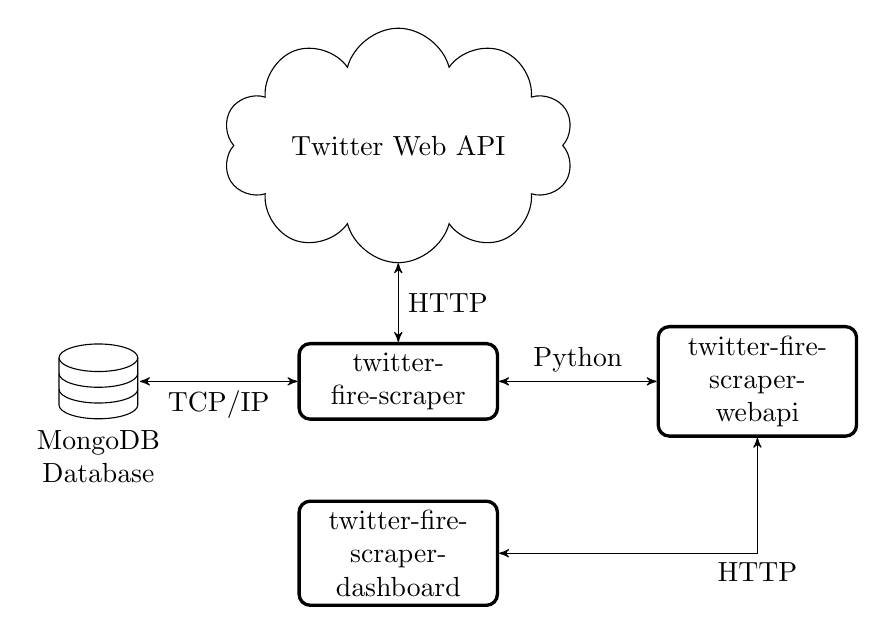
\begin{tikzpicture}[node distance=1cm, auto,]
        %nodes
        
        % Twitter Web API node
        \node[cloud, cloud puffs=10,aspect=2, draw]
        (twitterapi)
        {Twitter Web API}
        ;
        
        % twitter-fire-scraper node
        \node[plain, below=of twitterapi]
        (tfs)
        {twitter-fire-scraper}
        ;
        
        % database node
        \node[database, left=of tfs, xshift=-1cm,
        label={
            [align=center]
            below:MongoDB \\ Database
        },
        scale=2]
        (db)
        {}
        ;
        
        % twitter-fire-scraper-dashboard node
        \node[plain, below=of tfs]
        (tfs-dashboard)
        {twitter-fire-scraper-dashboard}
        ;
        
        % twitter-fire-scraper-webapi node
        \node[plain, right=of tfs, xshift=1cm]
        (tfs-web-api)
        {twitter-fire-scraper-webapi}
        ;
    
        % TFS and Twitter Web API
        \draw[<->] 
        (twitterapi) edge node 
            {HTTP}
        (tfs)
        ;
    
        % TFS and TFS-web-api
        \draw[<->]
        (tfs) edge node
            {Python}
        (tfs-web-api)
        ;
        
        % TFS and MongoDB database
        \draw[<->]
        (tfs) edge node
            {TCP/IP}
        (db)
        ;
        
        % TFS web api and TFS dashboard
        \draw[<->]
        (tfs-web-api) |- node
            {HTTP}
        (tfs-dashboard)
        ;
        
    \end{tikzpicture}
    % \includegraphics{}
    \caption{Application diagram}
    \label{fig:app_diagram}
\end{figure}

\subsection{Dashboard}

The dashboard component, called ``twitter-fire-scraper-dashboard''\footnote{\url{https://github.com/raaraa/IPRO497-Analytics-Team/tree/master/coding/twitter-fire-scraper-dashboard}}, works by querying a web API we have developed which allows a Node.js \footnote{\url{https://nodejs.org/}} web server to display a web interface for users to scrape and view tweets.

\subsection{Web API}

The web API component, called ``twitter-fire-scraper-webapi''\footnote{\url{https://pypi.org/project/twitter-fire-scraper-webapi/}}, exposes the functionality of our backend component to any applications which wish to consume the services it can provide over HTTP.

See figure \ref{fig:api_routes} for the routes that the web API serves.

\begin{figure}[H]
    \centering
    \begin{lstlisting}[language=Python]
[GET]
/info

[GET]
/scrape
    ?terms=["house fire","mudslide", {...}]
    &accounts=["@NWSChicago","@MABASIllinois", {...}]
    &count=3

[GET]
/scrape_terms
    ?terms=<"house fire","mudslide", {...}>
    &count=5

[GET]
/scrape_accounts
    ?accounts=<"@NWSChicago","@MABASIllinois", {...}>
    &count=200
    \end{lstlisting}
    \caption{API Routes}
    \label{fig:api_routes}
\end{figure}

\subsection{Backend}

The backend component, called ``twitter-fire-scraper''\footnote{\url{https://pypi.org/project/twitter-fire-scraper/}}, is a Python module which can send HTTPS reqeusts to Twitter's web API to retrieve, filter, and sort tweets from Twitter.

It has a variety of different tweet scraping filters that can be applied to it, such as location-based filtering, keyword-based filtering, and retweet-dependent filtering.

It facilitates saving scraped tweets to various sources, such as comma-separated value files, JSON files, and MongoDB databases.

It is designed to be used by programmers and data scientists, and thus simple to use yet powerful. This section contains demonstrations of how its interface can be used to perform scraping, collection, and saving of tweets.

\subsubsection{Scraping by keywords}

The first method that it can use to gather tweets is by keywords that the tweets contain. The scraper can take a single keyword and a count of results, or many keywords. Below is code showing the usage of the keyword-scraping feature:

\begin{lstlisting}[language=Python,caption=Scraping multiple keywords]
# Returns a total of 600 tweets
results = scraper.scrape_terms(
    terms={"fire", "#housefire", "firedamage"}, 
    count=200
)
\end{lstlisting}

This snippet of code will return 200 tweets each about the term ``fire'', the hashtag ``\#housefire'', and the term ``firedamage'' for a total of 600 tweets.

\subsubsection{Scraping by keywords restricted by location}

The next feature our scraper has is one which limits the areas that the scraper operates in. This is an augmentation of the scraper's ability to search for keywords and hashtags, and acts as a filter on that function.

This is important because most of the work that the ARC wishes to do takes place in or around Chicago.

Below is a code example of the same search, but restricted to within 50 miles of Chicago's center.

\begin{lstlisting}[language=Python,caption=Geo-location scraping filter]
# Returns 600 tweets that occur 50 miles from Chicago
results = scraper.scrape_terms(
    geocode="41.8297855,-87.666775,50mi",
    terms={"fire", "#housefire", "firedamage"}, 
    count=200
)
\end{lstlisting}

This time, we still get 200 tweets per term, but only ones that have been tagged within Chicago.

Instead of searching all of twitter for the three terms, only tweets that individuals have chosen to tag with a geographical location within a 50 mile radius of latitude 41.8, longitude -87.6, which is Chicago's center.

\subsubsection{Scraping by account}

This feature allows one to scrape the most recently tweeted tweets by one or more accounts.

This is to make it easy to repeatedly query accounts, or to get large amounts of tweets from a set of accounts.

Below is a code example of the scraper getting the top 100 tweets from various Twitter accounts that the  \@RedCross account follows.

\begin{lstlisting}[language=Python,caption=Scraping by account]
# Returns 300 tweets from 3 red cross accounts, 100 each.
results = scraper.scrape_accounts(
    accounts={"@RedCross", "@NWSChicago", "@MABASIllinois"},
    count=100
)
\end{lstlisting}

The syntax is very similar to that of the previous scraping methods. This snippet of code would result in a total of 300 tweets, 100 from each Twitter account.

\subsubsection{Saving to a CSV file}

This feature allows one to save scraped tweets to a comma-separated value file, to perhaps later be analyzed in a spreadsheet program like Microsoft Excel or be loaded into another data analysis program.

\begin{lstlisting}[language=Python,caption=Saving to CSV]
# Returns 300 tweets from 3 red cross accounts, 100 each.
results = scraper.scrape_accounts(
    accounts={"@RedCross", "@NWSChicago", "@MABASIllinois"},
    count=100
)

# Saves above results to a CSV file called 'output.txt'
scraper.save_statusdict_to_csv(results, 'redcross_tweets.csv')
\end{lstlisting}

\subsubsection{Other features}

The scraper allows you to scrape many more tweets than twitter normally allows you at any one time, and will wait when it hits the Twitter API rate limit\footnote{\url{https://developer.twitter.com/en/docs/basics/rate-limiting.html}} to finish scraping tweets.



\section{Conclusion}
``I always thought something was fundamentally wrong with the universe'' \citep{adams1995hitchhiker}

\bibliographystyle{plain}
\bibliography{references}
\end{document}
